
In this section we describe our approach in detail. Section~\ref{subsec-lw} defines our warping module, Section~\ref{subsec-lr} describes the label refinement module, and Section~\ref{subsec-alea} describes our noisy label learning approach.


\textbf{Problem Formulation}: We have a set of images $D_{I}$ and the corresponding labels $D_{L}$. We also have a set of images $D_{Iseq}$ consisting of images temporally adjacent to images in $D_{I}$. 
% Specifically, for each $I_{t}^{i} \in D_{I}$, the set of images $\{I_{t-x}^{i} | -p\leq x \leq p\}$ is a partition of $D_{Iseq}$. Here, $I \in \Bbb R ^{n \times w \times h}$, and the sub-script $t$ corresponds to temporal position in a video stream. 
Our goal is to generate the corresponding set of pseudo-labels, $\hat{D}_{Lseq}$. Using the generated pseudo-labels, our network can be trained on $D_{I}$ and $D_{Iseq}$, using corresponding labels from $D_{L}$ and $\hat{D}_{Lseq}$.

\subsection{Label Warping}
\label{subsec-lw}
The goal of this step is to generate warped labels $ \{\hat{L}^{w}_{n} | t\leq n \leq t + p\}$, where $p \in \mathbb{N}$ is a fixed integer, given the sequence of images $\{I_{n}| t\leq n \leq t + p\}$, and the annotated label $L_{t}$. In this step, we utilize a previous existing method~\cite{nvidia_cvpr19} for generating the warped labels. % We present a generalized formulation of this step.

% We now describe this system. 
% For the sake of simplicity, we drop the superscript $i$ denoting an image instance. 
We train a neural network $f_{\theta}$ such that, given a sequence of images $I_{t:t+x} = \{I_{n}| t\leq n \leq t + x\}$ it predicts parameters for the sampling and warping function $ \Phi$ to construct $I_{t+x}$ from $I_{t + x -1}$.
The pseudo-labels corresponding to $I_{t+x}$ can similarly be constructed by using the same function $\Phi$ on $\hat{L}^{w}_{t+x-1}$. For the sake of simplicity, we rewrite $I_{t:t+x}$ as the pair of images $(I_{t+x-1},I_{t+x})$. This step can be simply summarized as:

\begin{equation}
\label{eq-warp_gen}
    \Phi_{(t+x-1, t+x)} = f_\theta (I_{t+x-1}, I_{t+x}),
\end{equation}
\begin{equation}
\label{eq-warp_both}
    \hat{I}^{w}_{t+x} = \Phi_{(t+x-1, t+x)} ( \hat{I}^{w}_{t+x-1}) \quad;\quad \hat{L}^{w}_{t+x} = \Phi_{(t+x-1, t+x)} ( \hat{L}^{w}_{t+x-1}),
\end{equation}

where, we use $\hat{L}^{w}_t = L_t$ and $\hat{I}^{w}_t = I_t$. By using this method sequentially for $1 \leq x \leq p$, we can generate the warped labels $\hat{L}^{w}_{n}$ for all $t \leq n \leq t + p$.
This method exploits geometric information by predicting motion vectors for each pixel. A more detailed explanation can be found in~\cite{nvidia_cvpr19, sdc_net}. This method is prone to generating noisy labels due to errors in the estimation of the warping function $\Phi$. 

\textbf{Mask Inpainting}: We first introduce a simple post-processing step (named $\mathtt{MI}$) to enhance the warped labels, the goal being to identify regions where warping has failed, and to replace labels for such regions with other approximation strategies. 
% The presence of the reconstructed image $\hat{I^{w}}$, and the real image $I$ offers us a rather simple yet effective method to identify such regions. 
We measure the per-pixel distance between $\hat{I}$ and $I$ at each pixel $(x,y)$, and if it is higher than a fixed threshold $\tau$, we replace those labels with labels from a semantic segmentation network $S$ trained using $D_I$ and $D_L$. 
% This allows us to address propagation errors, and at the same time utilize semantic knowledge present in the annotated dataset. 
This is summarized as:

\begin{align}
\begin{split}
\label{eq-inpaint}
M(x, y) & = \mathbb{I}_{M}\big(d(\hat{I}(x,y),I(x,y) ) \leq \tau \big) \\
\hat{L}^{MI} & = \hat{L}^{w} \odot M + (1-M) \odot \hat{L}^{pred}
\end{split}
\end{align}
%The authors further propose \textit{joint-propagation}, replacing each $I_{t+1:t+p}$ in $D_{Iseq}$ with the warping based image reconstructions $\hat{I}_{t+1:t+p}$, given by equation~\ref{nvidia_main}, to gain more consistency between the pseudo-labels and images. This however is detrimental for the learning process as the distribution of constructed images $\hat{I_{t+1:t+p}}$ rapidly diverges from distribution of real images as we propagate further (refer figure~\cite{}).

where $d$ is a distance metric, $\tau \in \mathbb R$ is a fixed threshold, $\mathbb{I}_{M}$ is the indicator function, $L^{pred}$ represents the predicted labels from $S_\theta$ , and $\odot$ is the element-wise multiplication operator. While the labels are significantly improved after post-processing with $\mathtt{MI}$, they still contain noise, which burgeons as we propagate further. Additionally, the inpainted labels can frequently be wrong for classes where the segmentation network $S_\theta$ fails. 
% In the next section, we present the refinement module to address these drawbacks. 
For the sake of simplicity, we combine the steps \eqref{eq-warp_both} and \eqref{eq-inpaint}, and represent warping followed by post-processing with $\mathtt{MI}$, as $\Phi^{MI}$.

\let\clearpage\relax
\begin{figure}[t]
	\label{fig_method}
	\centering
	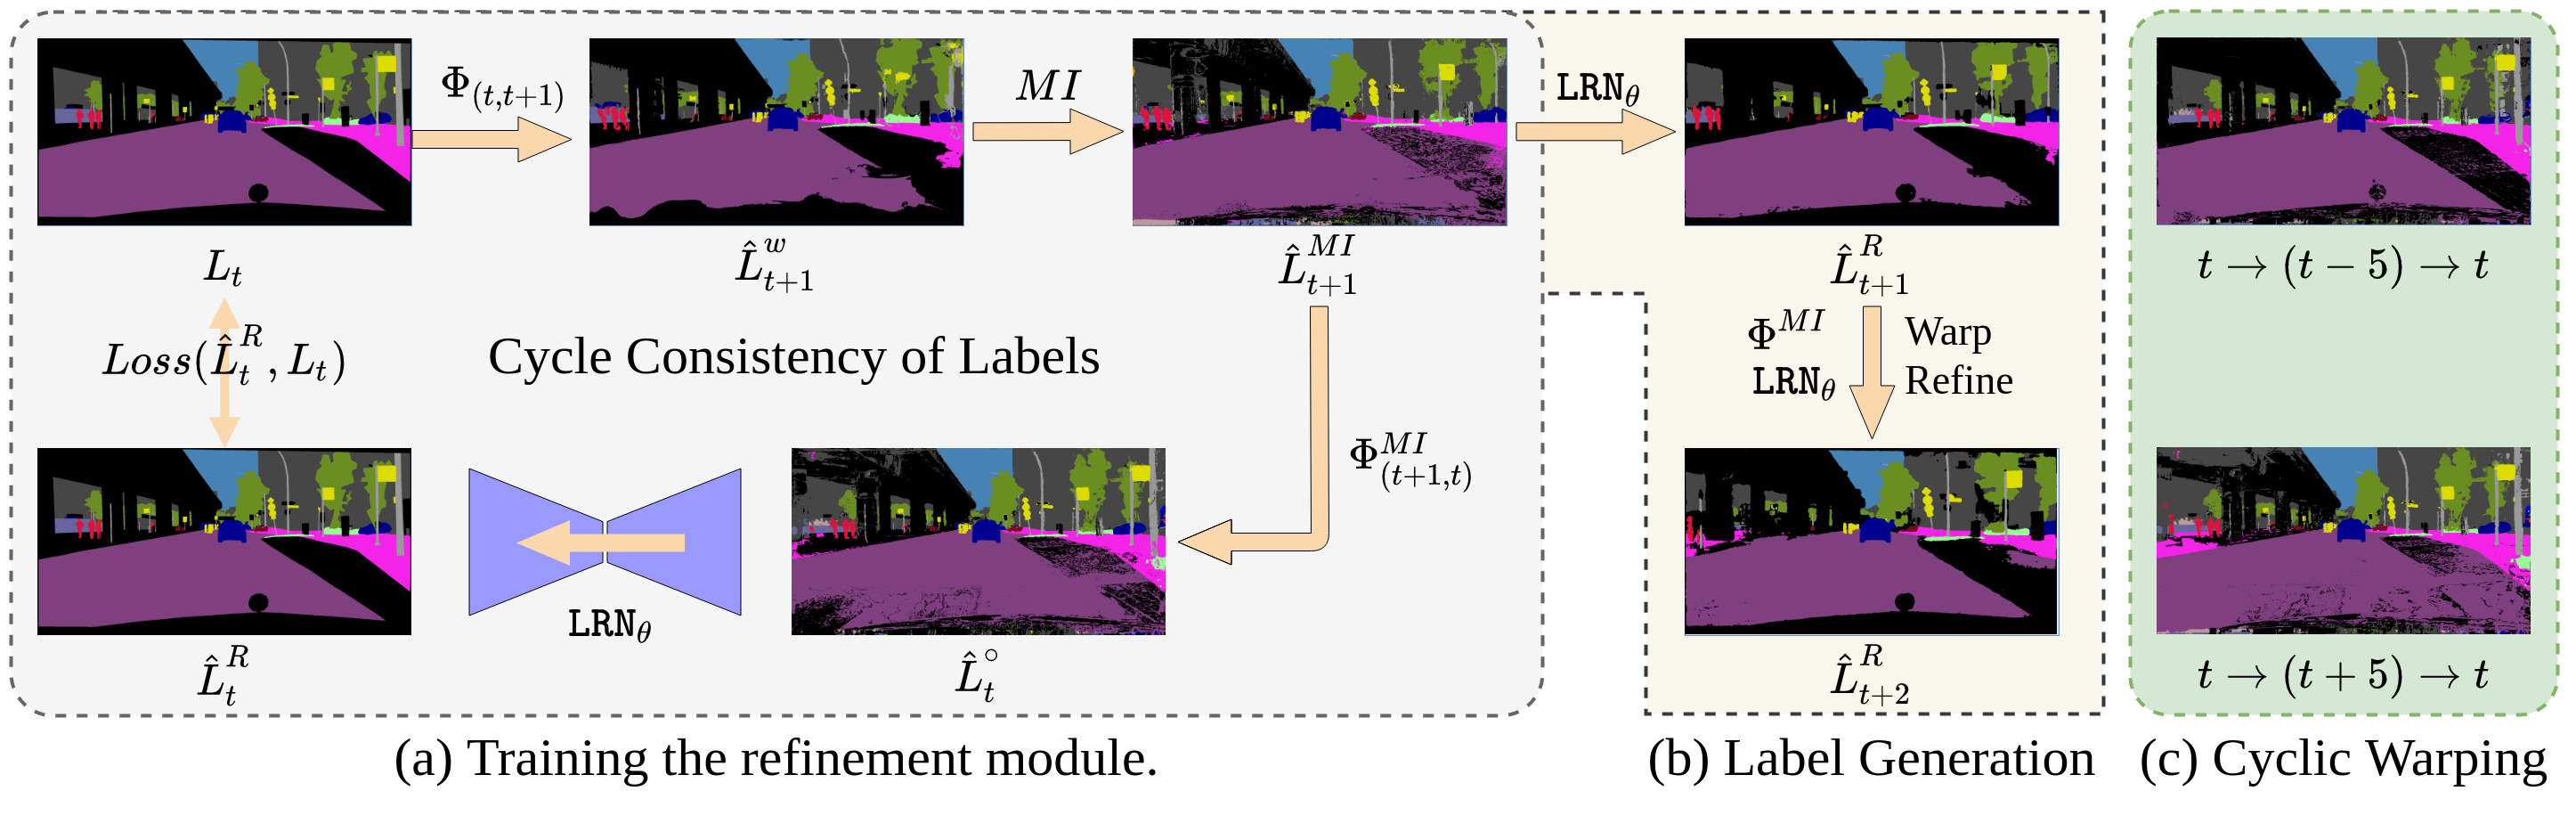
\includegraphics[width=1.0\linewidth]{figures/process_smaller_lr.png}
    \vspace{-2em}
	\caption{\small (a) For training $\texttt{LRN}_\theta$, the cyclic propagated labels $\hat{L}^{\circ}$ are used as input, as given by equation~\eqref{eq-cyclic-process}. (b) While generating labels, the warped post-processed labels $\hat{L}^{MI}$ are given as input to $\texttt{LRN}_\theta$. Iterative application of warping and refining is used to generate sequential labels. (c) The cyclic warped labels are generated for a wider range of cyclic loops to expose $\texttt{LRN}_\theta$ to more warping error while training.}
    \vspace{-1em}
\end{figure}



\subsection{Label Refinement}
\label{subsec-lr}

The warped post-processed labels $\hat{L}^{MI}$ need to be refined as they are still noisy. We do this by training a label refinement network ($\texttt{LRN}_\theta$), parameterized by $\theta$, which takes the pseudo-labels, the warped image, and the clean image, as input, and predicts the refined labels $\hat{L}^{R}$:
\begin{equation}
\label{eq-lrn_inference}
\hat{L}^{R} = \texttt{LRN}_{\theta}(\hat{L}^{MI}, \hat{I}^{w}, I)
\end{equation}

$\texttt{LRN}_\theta$ can be viewed as a denoising network, which takes the noisy samples $\hat{L}^{MI}$ and tries to predict the clean samples $L$. To train any denoising network, we typically need noisy-clean sample pairs. However, for ${t < n \leq t + p}$ we do not contain clean labels $L_{n}$ (as we do not have $D_{Lseq}$). Due to this, we do not have the noisy-clean samples $(L^{MI}, L)$ for training our refinement module. Hence, while using $\mathtt{LRN}_\theta$ is fairly simple, training it is non-trivial.

\textbf{Cycle Consistency of Labels:} With an ideal propagation mechanism, when a label $L_{t}$ is propagated through a cyclic loop in time (say $t$ to $t+1$ and then back to $t$), the resulting cyclic propagated labels (denoted by $\hat{L}^{\circ}_{t}$) should be consistent with initial labels $L_{t}$. Therefore, the inconsistency between $\hat{L}^{\circ}_{t}$ and $L_t$ reveal the modes of failure of the propagation mechanism. We utilize this inconsistency as the supervisory signal to train $\mathtt{LRN}_\theta$.
% \textbf{Cycle Consistency of Labels:} We posit that, with an ideal propagation method, when label $L_{t}$ is propagated through a cyclic loop (for example, $t$ to $t+1$, and then back to $t$), the resulting labels $\hat{L}_{t}$ should be consistent with the $L_{t}$. 
% We utilize this idea for learning how to refine warped labels $\hat{L}^{MI}$. Specifically, we utilize the inconsistency in cyclic propagation of labels as a supervisory signal to train $\mathtt{LRN}_\theta$.
First, we define the cyclic propagated labels $\hat{L}^{\circ}$ for a simple cyclic loop in time:
% If we warp the labels $L_t$ once forward($t$ to $t+1$, generating $\hat{L}^{w}_{t+1}$), and then warp $\hat{L}^{w}_{t+1}$ backwards ($t+1$ to $t$), we generate cyclic propagated labels $\hat{L}^{\circ}$:
% This operation is summarized in the following equations:
\begin{eqnarray}
% \begin{split}
\label{eq-cyclic-process}
    &\Phi_{(t, t+1)}  = f_\theta (I_t, I_{t+1}), \\
    &\hat{I}^{w}_{t+1} = \Phi_{(t, t+1)} (I_{t}) \quad ; \quad \hat{L}^{MI}_{t+1} = \Phi^{MI}_{(t, t+1)} ( \hat{L}^{w}_{t}) \\
    &\Phi_{(t+1, t)}  = f_\theta (\hat{I}^{w}_{t+1}, I_{t}), \\
\label{eq-cyclic}
    &\hat{I}^{\circ}_{t} = \Phi_{(t+1, t)} (\hat{I}^{w}_{t+1}) \quad ; \quad \hat{L}_{t}^{\circ} = \Phi^{MI}_{(t+1, t)} ( \hat{L}^{MI}_{t+1})
% \end{split}
\end{eqnarray}

These cyclic warped labels $\hat{L}_{t}^{\circ}$ contain artifacts created due to the warping process further exacerbated due to the multiple applications of the warping function $\Phi^{MI}$. 
Motivated by the concept of cycle consistency of labels, we utilize the pairs $( \hat{L}_{t}^{\circ},  L_{t})$  as the noisy-clean samples for training $\mathtt{LRN}_\theta$:
\begin{equation}
\label{eq-cyc-train}
% \begin{split}
    \hat{L}^{R} = \texttt{LRN}_\theta(\hat{L}^{\circ}, \hat{I}^{\circ}, I) \quad ; \quad   \theta^{*} = \underset{\theta}{\mathrm{argmin}}\;{ \mathbb{E}(\mathcal{L}(L^{R}, L))},
% \end{split}
\end{equation}
where $\mathcal{L}$ can be any standard loss function such as cross-entropy. In the process of learning to improve consistency between the cyclic warped labels $\hat{L}^{\circ}$ and $L$, $\texttt{LRN}_\theta$ also learns to refine single warped labels $L^{MI}$. It is important to note that cyclic labels, which capture the noise of the warping process, exist because $\Phi_{(t+1, t)} \neq \Phi^{-1}_{(t, t+1)}$.%  (which would otherwise lead to a trivial solution of $\hat{L}_{t}^{\circ} = L_t$). 


Equation~\eqref{eq-cyclic} represents the cyclic labels generated from a single forward and backward step. However, it is possible to perform multiple forward and backward steps, generating multiple $L^{\circ}_{t}$ for each $L_t$. This allows us to capture more diverse artifacts created due to $\Phi^{MI}$. Figure~\ref{fig_method} shows multiple cyclic warped samples for a given label $L_t$.
% We describe the architecture of $\texttt{LRN}_\theta$, inspired from~\cite{pix2pix}, in more details in the supplementary.

Once the refinement module is trained with the cyclic propagated label pairs, we propagate labels by a) warping, b) post-processing, and then finally c) refining with $\mathtt{LRN}_\theta$ to generate refined labels $\hat{L}^R_{t+p}$( refer equation~\eqref{eq-lrn_inference}). This is the complete pipeline of \emph{Warp-Refine Propagation}. At each time step $t+p$, the labels $\hat{L}^R_{t+p}$ undergo propagation to generate $\hat{L}^R_{t+p+1}$.
% This is given by:
% \begin{align}
% \begin{split}
% \label{nvidia_main}
%     \Phi_{(t+p, t+p+1)}  &= f_\theta (I_{t+p}, I_{t+p+1}), \\
%     \hat{L}^{MI}_{t+p+1} &= \Phi^{MI}_{(t+p, t+p+1)} ( \hat{L}^{R}_{t+p}) \\
%     \hat{L}^{R}_{t+p+1} &= LRN(\hat{L}^{MI}_{t+p+1},\hat{I}_{t+p+1}, I{t+p+1} )
% \end{split}
% \end{align}

\subsection{Uncertainty Aware Training}
\label{subsec-alea}

As shown in Figure~\ref{}, the \emph{Warp-Refine Propagation} pipeline generates pseudo-labels of high quality. While these are directly beneficial for training, we note that using labels propagated over a large temporal distance (say $t+10$) can lead to a drop in performance. This is due to the inherent noise in the pseudo-labels. It can be significantly advantageous if we can handle the noise, as psuedo-labels further away from the annotated frame contain novel information. 


%%%%%%%%%%%%%%%%%%%%%%%%%%%%%%%%%%%
%%%%%%%%%%%%%%%%%%%%%%%%%%%%%%%%%%%

% Formally, lets denote labels generated from a given data-generation pipeline as samples of distribution $P_{i}(y|x)$, where as the underlying label distribution is $P(y|x)$.
% % , and labels generated from propagation as samples of distribution $P_{p}(y|x)$. In our case, $D_{L}$ contains samples from $P_{m}(y|x)$, and $D_{\hat{L}seq}$ contains labels from $P_{p}(y|x)$.
% Using model $M_{\theta}(y|x)$, we estimate the distribution the underlying label distribution $P(y|x)$ by maximizing the expected log-likelihood of the model over the given data:
% \begin{equation}
%   \text{Objective} =  \underset{\theta}{\mathrm{argmax}} \big[ \mathbb{E}_{y\sim P(y|x)}\log M_{\theta}(y|x) \big] \sim  \underset{\theta}{\mathrm{argmax}} \sum_{i \in D}{\log M_\theta(y_i|x_i)}
% \end{equation}

% It is important to address the noise in the annotation process, especially in our case, where labels in $D_{Lseq}$ are highly noisy. It is inevitable that a Model which directly maximizes likelihood on $D_L$ and $D_{Lseq}$ under-performs on the test-set as deep networks have a high capacity to memorize noise in the training set[].

% We alleviate the harm caused by noise by modelling the aleatoric uncertainty from the given data. It has been shown that aleatoric uncertainty captures the uncertainty in the data generating process, e.g., inherent measurement noise, and can play a crucial role when training with noisy labels[].
% Specifically, we model $P_m$ and $P_p$ as follows:
% \begin{eqnarray}
%     y &=& \mu(x) + \eta_m \; {\textrm{where }}  y\sim P_m {\textrm{ and }} \eta_m \sim \mathcal{N}(0, \sigma_m^2(x)) \nonumebr \\ 
%     y &=& \mu(x) + \eta_p, \; {\textrm{where }}  y\sim P_p {\textrm{ and }} \eta_p \sim \mathcal{N}(0, \sigma_p^2(x))
% \end{eqnarray}
% Where, $\eta_m$ and $\eta_p$ represent the noise inherent to each annotation process. %Following [], we model $\eta_m$ and $\eta_p$ as additive Gaussian noise with distribution $\mathcal{N}(0, \sigma_m)$ and $\mathcal{N}(0, \sigma_p)$ respectively. 
% We adapt the model parameter $\theta$ specifies the statistics $(\mu^i, \sigma_m^i, \sigma_p^i)$ for each pixel $i$ in a given image $x$. The optimization objective can now be written as: 
% \begin{align}
% \begin{split}
%     %(\mu^i, \sigma_m^i, \sigma_p^i) &= M_{\theta}(x^i) \\
%     l_m^i |\theta \sim \mathcal{N}(\mu^i, \sigma_m^i) \quad &; \quad \hat{p^i_m} = \softmax(\hat{l^i_m}) \\
%     l_p^i |\theta \sim \mathcal{N}(\mu^i, \sigma_p^i) \quad &; \quad \hat{p^i_p} = \softmax(\hat{l^i_p}) \\
% \end{split}
% \end{align}
% \begin{equation}
%     \text{Objective} =  \underset{\theta}{\mathrm{argmax}} \Bigg[ \sum_{m \in D_L}{\log E_{\hat{l^i_m} \sim  \mathcal{N}(\mu^i, \sigma^i_m)}(\hat{p^i_m})} + \sum_{p \in D_{Lseq}}{\log E_{\hat{l^i_p} \sim  \mathcal{N}(\mu^i, \sigma^i_p)}(\hat{p^i_p})} \Bigg]
% \end{equation}

% \let\clearpage\relax
% 
%%%%%%%%%%%%%%%%%%%
%%% SVHN RESULTS
%%%%%%%%%%%%%%%%%%%
\begin{figure}[t]
\begin{center}\small
\setlength{\tabcolsep}{3pt}
		\subfigure[Mean IOU of various propagation methods.]
		{
			\begin{minipage}{0.58\textwidth}
				\label{fig:input-model}
				% \centering
				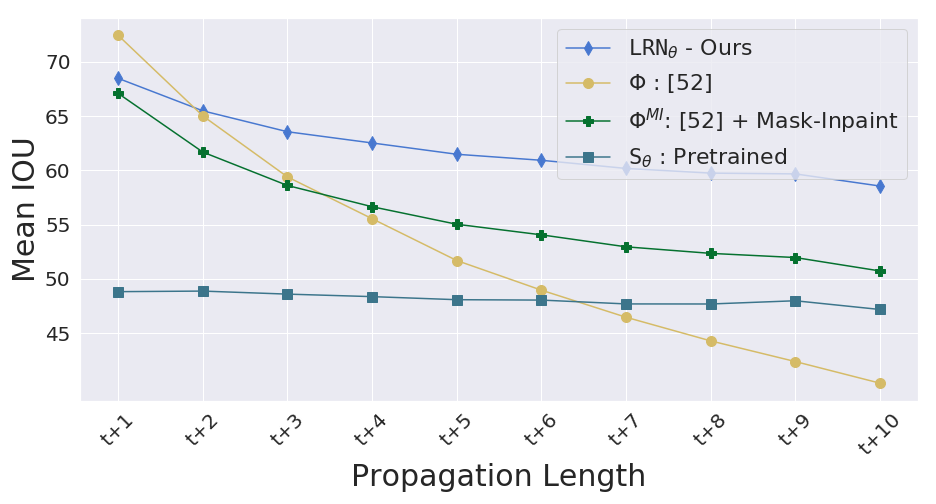
\includegraphics[width=1.0\linewidth]{figures/miou_apollo.png}
				\hfill
				\vfill
			\end{minipage}
		}
% \hspace{-1em}
% \vtop{
% \vspace{-1em}
\hfill
% \hbox{
% 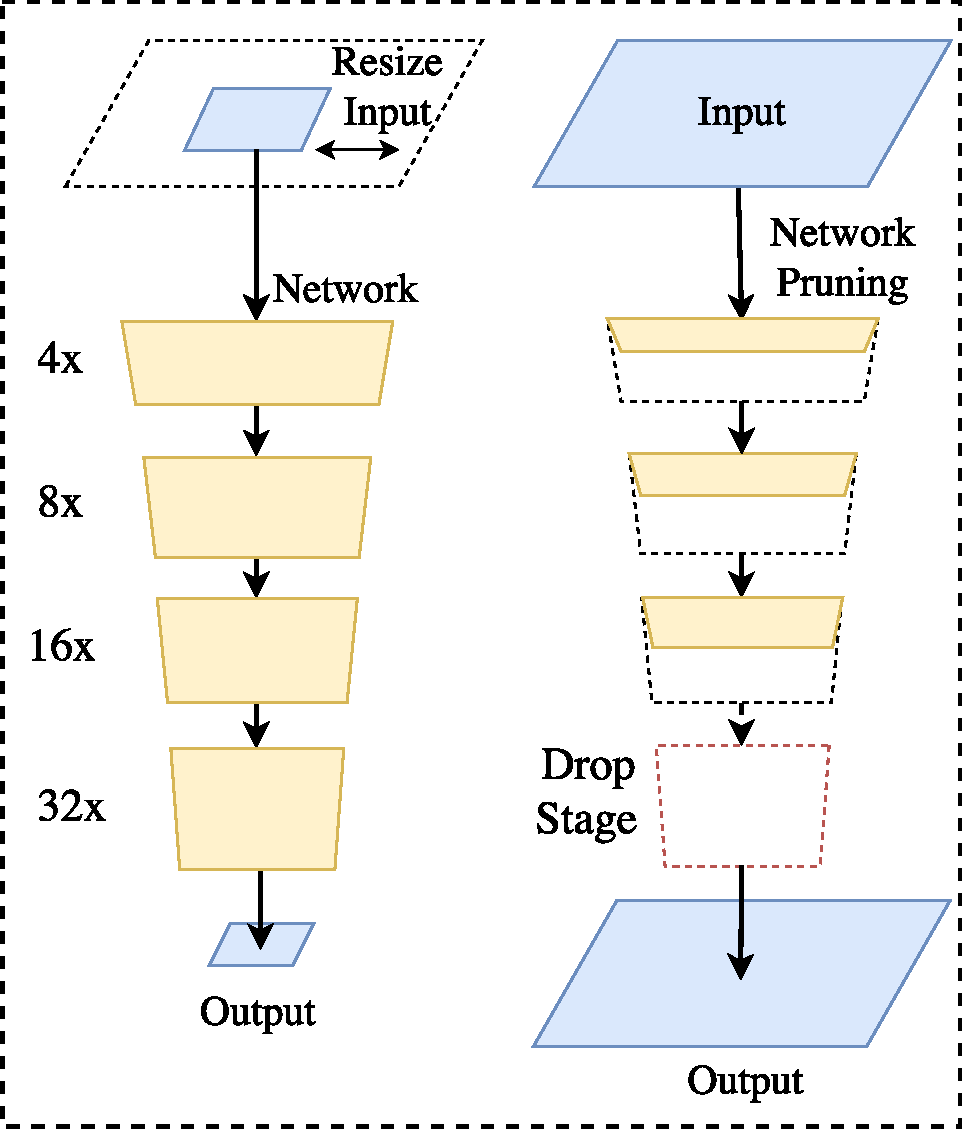
\includegraphics[width=0.6\textwidth]{figures/input_model.pdf}
		\subfigure[Qualitative Example]{
            \begin{minipage}{0.35\textwidth}
                \centering
				\label{fig:input-model}
				% \centering
				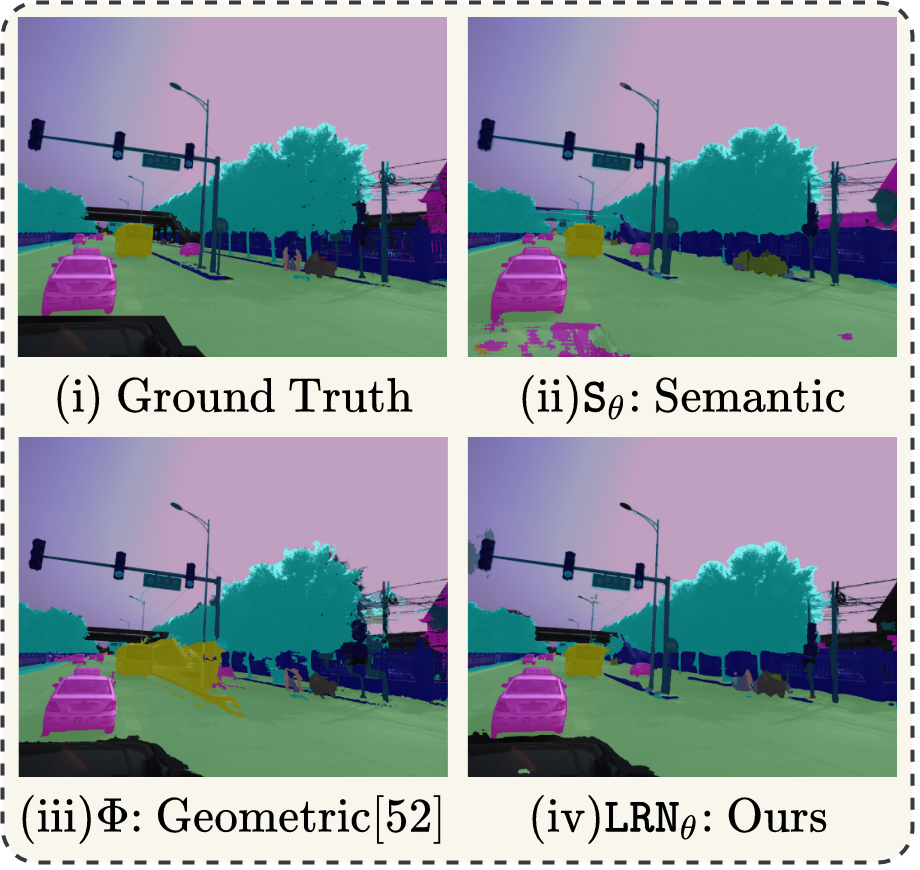
\includegraphics[width=1.0\linewidth]{figures/apollo_vis.png}
\end{minipage}
% }}%
}
\end{center}
\vspace{-1em}
\caption{\small \emph{(a)} We \textit{quantitatively} show that our method is significantly better than previous \textit{state-of-the-art} method. \emph{(b)} \cite{nvidia_cvpr19}, which uses geometric information is suspectible to poor warping, on the other hand generating pseudo-labels from semantic predictions (via network $\mathtt{S}_\theta$ poorly labels rare classes. Our method combines geometric and semantic information together, generating cleaner labels.}
\label{table:svhn}

		\vspace{-1em}
\end{figure}

% where $p_i$ represents the probability vector. 
% Due to the lack of analytical solution for $E(p_i)$, we approximate the object by monte carlo integration as described in []. This entails drawing $t$ samples from the distribution  $\mathcal{N}(\mu^i, \sigma^i)$ and calculating the empirical mean probability vector $p^i$ at each pixel. As both the data generation process noises $\eta_m$ and $\eta_p$ are modelled as zero-mean Gaussian noises, $\softmax(\mu^i)$ models the underlying distribution $P(y|x)$. Hence at test-time, our predictions for a given image is simply $\mu^i$ for each pixel $i$ in the image.

% In practice, this objective simply means that we model separate aleatoric uncertainty for each of label dataset $D_L$ and $D_{Lseq}$. We add a two small heads to the given segmentation models to predict $\sigma_m$ and $\sigma_p$, and while calculating the loss, if the label is from $D_L$ we utilize the $\sigma_m$ , if the label is from $D_{Lseq}$ we utilize $\sigma_p$. In section~\ref{} we show the benefits of this approach over previous methods, as well as over modelling a single aleatoric uncertainty for the combined dataset $D_L$ and $D_{Lseq}$.

% % FOR Experiements
% \subsection{Different Narrative}

%%%%%%%%%%%%%%%%%%%%%%%%%%%%%%%%%%%%%%%%%%
%%%%%%%%%%%%%%%%%%%%%%%%%%%%%%%%%%%%%%%%%%%

Formally, let us denote labels generated from a given noisy data-generation process $\delta$ as samples of distribution $P_{\delta}(y|x)$, whereas the underlying label distribution is $P(y|x)$.
% , and labels generated from propagation as samples of distribution $P_{p}(y|x)$. In our case, $D_{L}$ contains samples from $P_{m}(y|x)$, and $D_{\hat{L}seq}$ contains labels from $P_{p}(y|x)$.
Typically, using model $M_{\theta}(y|x)$ parameterized by $\theta$, we estimate the underlying label distribution $P(y|x)$ by maximizing the expected log-likelihood of the model over the given data:
\begin{equation}
   \theta^{*} =  \underset{\theta}{\mathrm{argmax}} \big[ \mathbb{E}_{y\sim P(y|x)}\log M_{\theta}(y|x) \big] \sim  \underset{\theta}{\mathrm{argmax}} \sum_{i \in D}{\log M_\theta(y_i|x_i)},
\end{equation}
where $\theta^{*}$ represents the optimal parameters for $M_\theta$. Since we contain noisy samples from $P_{\delta}$, our model is biased to model $P_{\delta}$, rather than $P$. To address the distributional shift between $P_\delta$ and $P$ we modify the objective of our optimization. 
Let us consider the relation between noisy labels and clean labels as $P(y_\delta|x,y)$, where $y_\delta$ represents the noisy sample for a given $x$. Since we want $M_\theta$ to model the underlying label distribution $P$, we can rewrite our estimate $P_\theta$ for noisy labels $y_\delta$, and the corresponding objective as:
% \begin{eqnarray}
% \begin{split}
%     P(y_\delta|x) &= \sum_{y'}P(y_\delta | x, y')P(y=y'|x), \\  
%     P_\theta(y_\delta|x) &= \sum_{y'}(P(y_\delta | x, y')+\Delta(y_\delta | x, y'))M_\theta(y=y'|x) \label{eq:noisy distribution}
% \end{split}
% \end{eqnarray}
\begin{equation}
    P(y_\delta|x) = \sum_{y'}P(y_\delta | x, y')P(y=y'|x) \quad ; \quad P_\theta(y_\delta|x) = \sum_{y'}(P(y_\delta | x, y'))M_\theta(y=y'|x)
\label{eq:noisy distribution}
\end{equation}
\begin{equation}
%   \text{Objective} \sim  \underset{\theta}{\mathrm{argmax}} \big[ \sum_{y_\delta \sim P_\delta}{\log \sum_{y'}P(y_\delta|x_i, y')M_\theta(y'| x_i)} \big]
   \theta^{*} \sim  \underset{\theta}{\mathrm{argmax}} \big[ \sum_{y_\delta \sim P_\delta}{\log P_\theta(y_\delta | x)} \big]
   \label{eq_new_object}
\end{equation}

\begin{theorem}
\label{thm:dtv bound}
Let $\epsilon = 1-\min_{y'}P(y_\delta=y' | x, y')$.
If $\epsilon < 0.5$, then the following inequality holds for the distributions $P(y_\delta|x)$ and $P_\theta(y_\delta|x) $ defined in Eq.\eqref{eq:noisy distribution}.
\begin{align}
    d_{TV}(P(y|x), M_\theta(y|x)) \leq 
    \frac{1}{1-2\epsilon}
    \left(\sqrt{2KL[P(y_\delta|x)|P_\theta(y_\delta|x)]}
    + \gamma  \right).\label{eq:dtv_bound}
\end{align}
where $d_{TV}(p(y),q(y))$ is the total variation distance and $KL[p(y)|q(y)]$ is the Kullback-Leibler divergence.
% where $\gamma = \frac{1}{2}\sum_{\hat{y}}|\sum_y \Delta(\hat y|y,x)M_\theta(y|x)|$, $d_{TV}(p(y),q(y)) = \frac{1}{2}\sum_y |p(y)-q(y)|$ is a total variation distance and $KL[p(y)|q(y)] = \sum_y p(y)\log\frac{p(y)}{q(y)}$ is a Kullback-Leibler divergence.
\end{theorem}

% Need to update theorem to be without reference to \Delta. 
Therefore, our objective~\eqref{eq_new_object} which minimizes the KL-divergence between $P(y_\delta|x)$ and $P_\theta(y_\delta|x)$, lowers the total variation distance between  $P(y|x)$ and $M_\theta(y|x)$ as well. The proof is provided in the supplementary.

% When $\Delta(y_\delta | x, y')=0$, 
% Theorem 1 implies that we can completely minimize the total variation distance between the true label distribution $P(y|x)$ and model distribution $M_\theta(y|x)$ through the learning of the noisy label distribution $P(y_\delta|x)$ 
% by using the model $P_\theta(y_\delta|x)$ 
% as long as $\min_{y'}P(y_\delta=y' | x, y') > 0.5$.
% On the other hand, when $\Delta(y_\delta | x, y')$ is nonzero, we can minimize the total variation distance only up to the constant $\frac{\gamma}{1-2\epsilon}$.

%In the supplementary, we prove that minimizing the KL-divergence between $P(y_\delta|x)$ and $P_\theta(y_\delta|x)$ minimizes the total variation distance $d_{TV}$ between  $P(y|x)$ and $M_\theta(y|x)$. 
% Formally: 
% \begin{equation}
%     d_{TV} (P(y|x),M(y|x)) \leq KL_D(P(y_\delta|x),P_\theta(y_\delta|x))
% \end{equation}
% Note that our proof is for a known relation $P(y_\delta |x, y )$, in practice, we use only an estimate $\hat{P}(y_\delta |x, y)$. 
Note that our formulation is independent of the labelling process $\delta$, and hence can be used for multiple labelling processes $\delta_j; j \in \mathbb{N}$.
% Let us denote $P_\theta(y_{\delta_0} | x) = M_\theta(y|x)$ by assuming the manual annotation is also a kind of noisy labeling process.
Now, we model $P_\delta$ and as a noisy version of $P$. Taking inspiration from~\cite{gal_main}, 
we represent $P_\theta(y_{\delta_j} | x)$ as:
%for a given labelling process $\delta_j$ we model the relation between clean and noisy labels as:
\begin{align}
    P_\theta(y_{\delta_j} = k | x) &= E_{a^{i}_{j,k} \sim \mathcal{N}(\mu^i_k(x), \sigma_{\delta_j}^i(x))}[\softmax(a^{i}_{j,k})]
\end{align}
where $\softmax(a_k) = \exp(a_k)/\sum_{k'}\exp(a_{k'})$ is the softmax function.
% \begin{equation}
%     y_{\delta_j} = y + \eta_{\delta_j} \; {\textrm{where }}  y_{\delta_j} \sim P_{\delta_j}, y \sim P(y|x){\textrm{ and }} \eta_{\delta_j} \sim \mathcal{N}(0, \sigma_{\delta_j}^2(x))
% \end{equation}
% Where, $\eta_{\delta_j}$ represent the noise inherent to each labelling process $\delta_j$ (the relation $P(y_{\delta_j}| x, y)$ is modelled by the additive Gaussian noise $\eta_{\delta_j}$).% (hence P()). %Following [], we model $\eta_m$ and $\eta_p$ as additive Gaussian noise with distribution $\mathcal{N}(0, \sigma_m)$ and $\mathcal{N}(0, \sigma_p)$ respectively. 
We adapt the model parameter $\theta$ to model the statistics $(\mu^i(x), \sigma_{\delta_0}^i(x),\sigma_{\delta_1}^i(x), .. )$ for each pixel $i$ in a given image $x$. The optimization objective can now be written as: 
% \begin{align}
% \begin{split}
%     %(\mu^i, \sigma_m^i, \sigma_p^i) &= M_{\theta}(x^i) \\
%     l_{\delta_j}^i |\theta \sim \mathcal{N}(\mu^i, \sigma_{\delta_j}^i) \quad &; \quad \hat{p^i_{\delta_j}} = \softmax(\hat{l^i_{\delta_j}}) \\
% \end{split}
% \end{align}
\begin{equation}
    % \text{Objective} =  \underset{\theta}{\mathrm{argmax}} \Bigg[ \sum_{\delta_j}{\sum_{i \in D_{{\delta_j}}}{\log \mathbb{E}_{\hat{l^i_{\delta_j}} \sim  \mathcal{N}(\mu^i, \sigma^i_{\delta_j})}(\hat{p^i_{\delta_j}})}} \Bigg]
    \theta^{*} =  \underset{\theta}{\mathrm{argmax}} \Bigg[ \sum_{j}{\sum_{i \in D_{{\delta_j}}}{\log P_\theta(y_{\delta_j} | x)}} \Bigg]
\end{equation}

\let\clearpage\relax

%%%%%%%%%%%%%%%%%%%
%%% SVHN RESULTS
%%%%%%%%%%%%%%%%%%%
\begin{figure}[t]
\begin{center}\small
\setlength{\tabcolsep}{3pt}
		\subfigure[Mean IOU of various propagation methods.]
		{
			\begin{minipage}{0.58\textwidth}
				\label{fig:input-model}
				% \centering
				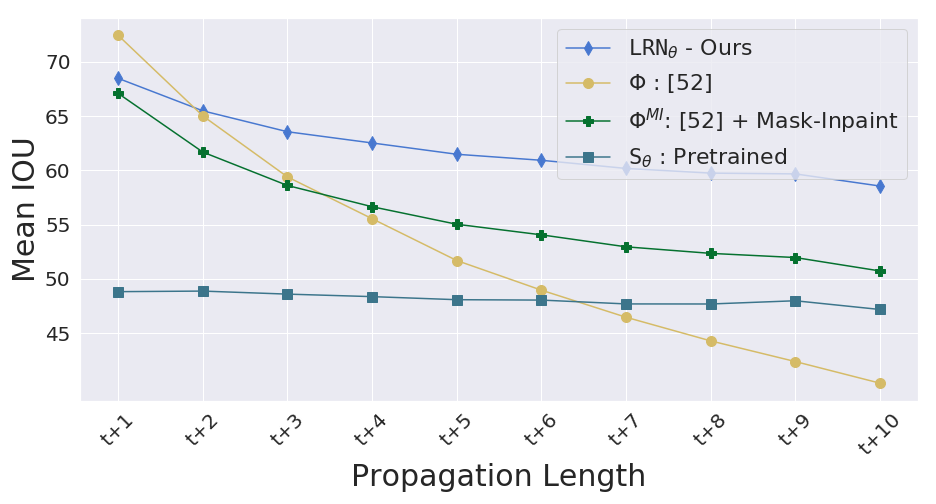
\includegraphics[width=1.0\linewidth]{figures/miou_apollo.png}
				\hfill
				\vfill
			\end{minipage}
		}
% \hspace{-1em}
% \vtop{
% \vspace{-1em}
\hfill
% \hbox{
% 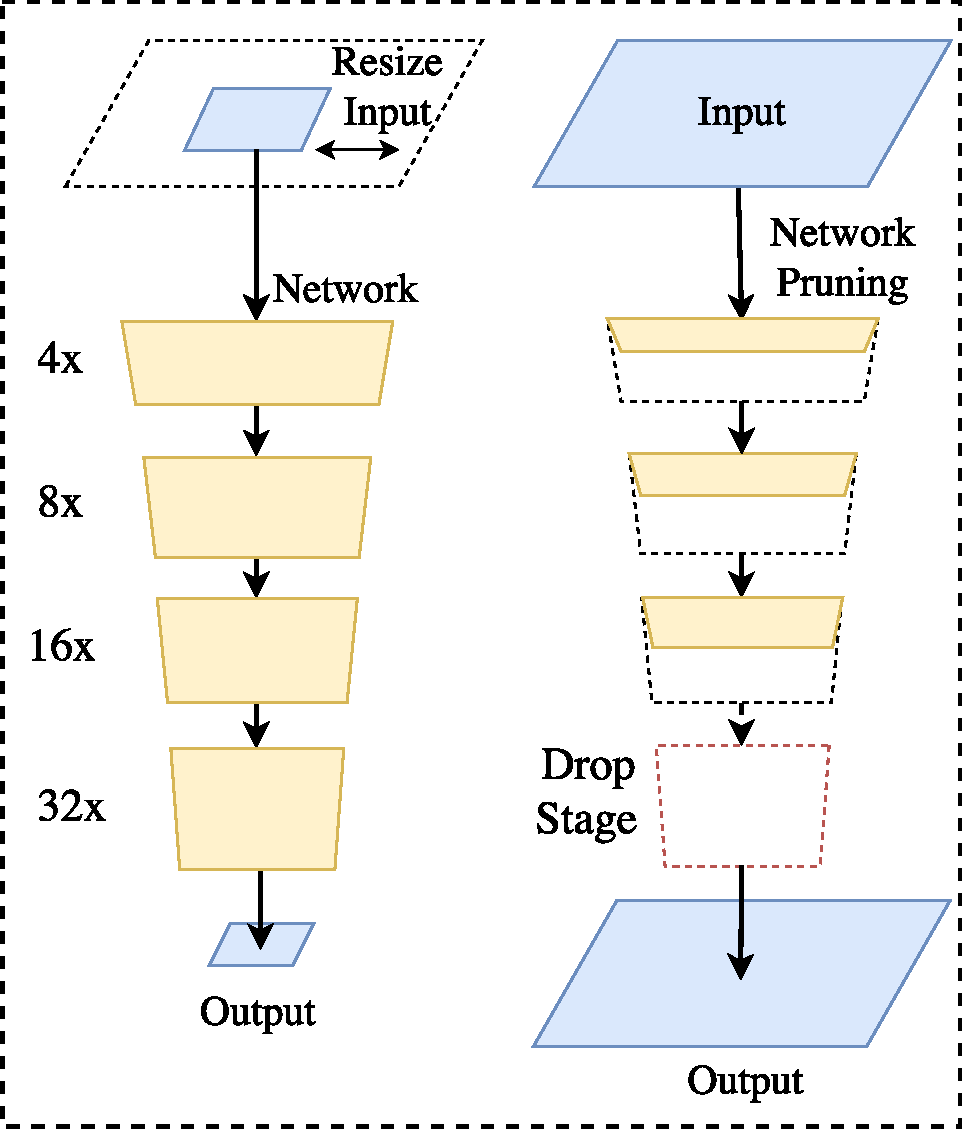
\includegraphics[width=0.6\textwidth]{figures/input_model.pdf}
		\subfigure[Qualitative Example]{
            \begin{minipage}{0.35\textwidth}
                \centering
				\label{fig:input-model}
				% \centering
				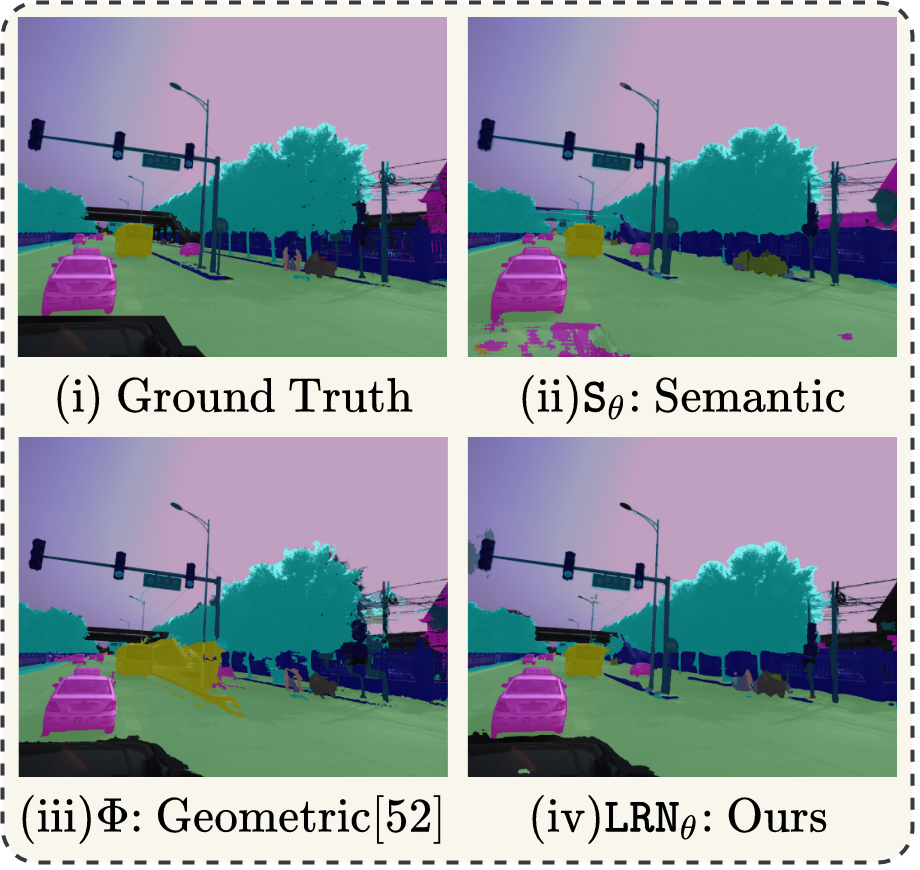
\includegraphics[width=1.0\linewidth]{figures/apollo_vis.png}
\end{minipage}
% }}%
}
\end{center}
\vspace{-1em}
\caption{\small \emph{(a)} We \textit{quantitatively} show that our method is significantly better than previous \textit{state-of-the-art} method. \emph{(b)} \cite{nvidia_cvpr19}, which uses geometric information is suspectible to poor warping, on the other hand generating pseudo-labels from semantic predictions (via network $\mathtt{S}_\theta$ poorly labels rare classes. Our method combines geometric and semantic information together, generating cleaner labels.}
\label{table:svhn}

		\vspace{-1em}
\end{figure}

%where $p^i$ represents the probability vector. 
Due to the lack of analytical solution for $ P_\theta(y_{\delta_j} | x)$, %  $\mathbb{E}(p^i)$, 
we approximate the objective by Monte Carlo integration as described in~\cite{gal_main}. %This entails drawing $t$ samples from the distribution  $\mathcal{N}(\mu^i, \sigma^i)$ and calculating the empirical mean probability vector $p^i$ at each pixel. 
% As all the data generation process noises $\eta_{\delta_j}$ are modelled as zero-mean Gaussian noises, 
As $\softmax(\mu^i)$ models the underlying distribution $P(y|x)$, at test-time, our predictions for a given image is simply $\mu^i$ for each pixel $i$ in the image.

In practice, this objective translates to modelling separate aleatoric uncertainty components for each of the noisy labelling processes $\delta_j$. The aleatoric uncertainty is modelled by adding a small two-layer head to the given segmentation models to predict $\sigma_{\delta_j}$. In Section~\ref{section-exp}, we show the benefits of this approach over modelling a single aleatoric uncertainty for the combined dataset.

\textbf{Using Pseudo Labels}: We also utilize pseudo-semantic labelling~\cite{taskonomy2018, pseudo_nips_1} for data points where label propagation is not possible. For Cityscapes~\cite{cs_dataset}, we use predictions from a model $S_\theta$ trained utilizing only the labels $D_L$, to create dataset $D_{\hat{L}ps}$ (specifically, labels for the \texttt{train\_extra} subset of Cityscapes). As our training procedure is agnostic to the label generation process, we can use the different labels by simply modelling a separate uncertainty parameter $\sigma_{\delta_j}$ for each of them. 
% $D_L$, $D_{\hat{Lseq}}$ and $D_{\hat{L}ps}$ to train our final model by simply modelling the three noise processes $\eta_L$, $\eta_{\hat{Lseq}}$ and $\eta_{\hat{L}ps}$ respectively.

% \begin{equation}
%     log E_{\hat{l_i} \sim  \mathcal{N}(u_i, \sigma_i)}(\hat{p_i}) \sim log(\frac{1}{T}\sum_{t}{\text{soft}_{\text{max}} (u_i + \epsilon_t * \sigma_i)}
% \end{equation}
% The problem with [below para] is that while our objective/modelling changed, there is no guarentee that is what will happen inside. Also it makes it hard to get to why a sigma for clean labels. However, if we start from Aleatoric, and then highlight this feature in discussions, we can make the link to generic noisy augmentation processes. 


% To address this mismatch between the objective and the optimization process, we change our optimization process. Specifically, we introduce a parameterized model $M_\beta$ to model the distribution $P(y_\delta|x, y)$ where $y \sim P(y|x)$ and $y_\delta \sim P_\delta(y|x)$. This model tries to estimate the conditional distribution of the noisy labels, given the clean labels, and corresponding image $x$. Hence, our learning objective becomes:

% Modelling the noise $\eta$ is a parameterized modelling of $P(y_\delta|x,y)$. It can be seen as a separate model $M_\beta$, with the final objective:
% \begin{equation}
%     M_{(\theta, \beta)} \sim  \underset{(\theta, \beta)}{\mathrm{argmax}} \big[ \sum_{y_m \in D_L}{\log M_\theta(y_m|x_m)} + \sum_{y_{n\delta} \in D_{Lseq}}{\log (M_\beta(y_{n\delta}|x_n,y_n)  M_\theta(y_n|x_n)) \big]}
% \end{equation}



